% Main Thesis File: This is the main file and it connects all the different parts of the thesis and compiles it into a single outcome file.

\documentclass[onecolumn, 12 pt, doublespace, fullpage, a4paper]{report}
\renewcommand{\baselinestretch}{1.75} % baseline stretch

% Packages
\usepackage{amssymb}
\usepackage{amsthm}
\usepackage[cmex10]{amsmath}
\usepackage{adjustbox} 
\usepackage{arabtex} 
\usepackage{academicons}
\usepackage{breakcites} 
\usepackage{color}
\usepackage{epsfig}
\usepackage{epstopdf}
\usepackage{etoolbox}
\usepackage{enumitem}
\usepackage{float}
\usepackage{fancyhdr}
\usepackage{graphicx}
\usepackage{graphics}
%\usepackage{hyperref} % if you want to highlight the links
\usepackage[hidelinks]{hyperref}
\usepackage{latexsym,amsfonts}
\usepackage{longtable}
\usepackage{listings}
\usepackage{lscape} 
\usepackage{lipsum}
\usepackage{multirow}             
\usepackage{pdfpages}
\usepackage[figuresright]{rotating} 
\usepackage{sectsty}
\usepackage{setspace}
\usepackage{subfigure}
\usepackage{textcomp}
\usepackage{utf8} 
\usepackage{url} 
\usepackage{wrapfig} 
\usepackage{wasysym} 
\usepackage{xcolor}


% you can define your most used synonyms/acronyms
\def\KAUST {King Abdullah University of Science and Technology}
\def\dg{$^\circ$}		 % for degree celcius
\def\2{$^2$}			 % for raised to power 2
\def\3{$^3$}			 % for raised to power 3
\def\-2{$^{-2}$}		 % for raised to power -2
\def\-3{$^{-3}$}		 % for raised to power -2
\def\-1{$^{-1}$}		 % for raised to power -1
\def\h{W.m$^{-2}$K$^{-1}$}
\def\hh{kJ.kg$^{-1}$}
\def\hfg{kJ.kg$^{-1}$}
\def\ss{kJ.kg$^{-1}$K$^{-1}$}
\def\Q{W.m$^{-2}$}
\def\mone {$^{-1}$}
\def\mtwo {$^{-2}$}
\def\um{$\mu m$}
\def\kwhm{kWh.m$ ^{-3} $}
\def\LMH{kg.m$^{-2}$h$^{-1}$}


% Changing chapters' headings and subheadings to size 14
\chapterfont{\fontsize{14}{15}\selectfont}   % font size and baseline stretch
\sectionfont{\fontsize{14}{15}\selectfont}
\subsectionfont{\fontsize{14}{15}\selectfont}
\subsubsectionfont{\fontsize{14}{15}\selectfont}

       
\pagestyle{fancy} % adds a line at the top of every page, except title-page
\fancyhead{} \fancyfoot{} % for header and footer
\fancyhead[CO,CE]{\thepage}    % center odd and even page number

%centering the page numbers with text body
\fancyheadoffset[L]{0.01mm}
\renewcommand{\headrulewidth}{0pt}


%The following code changes the empty vertical space above a new chapter title. It sets it from 50pt to 20pt
\makeatletter
\patchcmd{\@makechapterhead}{50\p@}{20pt}{}{}
\patchcmd{\@makeschapterhead}{50\p@}{20pt}{}{}
\makeatother
%end of modification



% The following code redefines the plain pagestyle with the objective of moving the page number from the bottom to the top of the page. This only affects new chapter pages.
\fancypagestyle{plain}{
\fancyhf{} %clear all header and footer fields
\fancyhead[C]{\thepage} %puts number on top center of the page
\renewcommand{\headrulewidth}{0pt}
\renewcommand{\footrulewidth}{0pt}}
%ending of plain pagestyle modification.




% ### Nomenclature, List of Abbreviations and List of Symbols 
   \usepackage{ifthen,xkeyval,xfor,amsgen}
   \usepackage[acronym,toc, nogroupskip]{glossaries}
   \newglossary[slg]{symbols}{syi}{sbl}{List of Symbols}
 
   \makeglossaries
   
   \include{Lists}
   % Run the following three lines in the command line to get the lists
%makeindex -s Thesis.ist -t Thesis.alg -o Thesis.acr Thesis.acn
%makeindex -s Thesis.ist -t Thesis.slg -o Thesis.syi Thesis.sbl
%makeindex -s Thesis.ist -t Thesis.glg -o Thesis.gls Thesis.glo

% ### End of addition




% Modified commands
\newcommand{\Tab}{\hspace{2ex}}
\usepackage[lmargin=40mm, rmargin=25mm, vmargin=25mm, headsep=2.5mm]{geometry}
\newcommand{\mathsym}[1]{{}}
\newcommand{\unicode}[1]{{}}
\renewcommand{\thechapter}{\arabic{chapter}}
\renewcommand\bibname{\centering BIBLIOGRAPHY}
%\newcommand{\orcid}[1]{\href{https://orcid.org/#1}{\textcolor[HTML]{A6CE39}{\aiOrcid}}}



\begin{document}

% $$$$$$$$$$$$$$$$$  Start of Thesis Front matter   $$$$$$$$$$$$$$

%\vspace{10mm}  % vertical space
\thispagestyle{empty}
\addvspace{5mm}  % vertical space until length

%$$$$$$$$$$$$$$$$$$$$$$$$$$$$$$$$$$$$$$$$$$$$$$$$$$$$$$$$$$$$$$$$$$$$$$$$$$$$$$$$$

% make the title page
\begin{center}
\begin{doublespace}
{\textbf{{\large Engineering Math Final On AlexNet}}}%\vfill % Write your thesis title
\end{doublespace}

\vspace{10mm}
{Paper by}\\
{Dov Cattan} %\vfill

\vspace{30mm}

{Engineering Math (MAP 3305)}\\[12pt]
{Computer Engineering}\\[12pt]
{Bachelors of Science} \vfill
{Florida Atlantic University }\\
{Boca Raton, FL, USA}
\vfill


%\maketitle
\begin{onehalfspace}
{\copyright May,2022}\\
Dov Cattan\\               % write your First name second name
All rights reserved\\


\end{onehalfspace}

\end{center}
% end of title page
%$$$$$$$$$$$$$$$$$$$$$$$$$$$$$$$$$$$$$$$$$$$$$$$$$$$$$$$$$$$$$$$$$$$$$$$$$$$$$$$$$
\newpage

%$$$$$$$$$$$$$$$$$$$$$$$$$$$$$$$$$$$$$$$$$$$$$$$$$$$$$$$$$$$$$$$$$$$$$$$$$$$$$$$$$




\begin{onehalfspacing}%To make the table of contents, figures, and tables single spaced, as required by the formatting guidelines, pg. 24.

\renewcommand{\contentsname}{\centerline{\textbf{{\large TABLE OF CONTENTS}}}}
\tableofcontents


\printglossary[type=\acronymtype,style=long3col, title=\centerline{LIST OF ABBREVIATIONS}, toctitle=List of Abbreviations, nonumberlist=true] 

\printglossary[type=symbols,style=long3col, title=\centerline{LIST OF SYMBOLS}, toctitle=List of Symbols, nonumberlist=true]




\end{onehalfspacing}
% \printglossary[style=altlist,title=Nomenclature, toctitle=Nomenclature, nonumberlist=true] 

% $$$$$$$$$$$$$$$$$  Thesis front matter ends   $$$$$$$$$$$$$$



% $$$$$$$$$$$$$$$$$  include your separate chapters   $$$$$$$$$$$$$$
\chapter{Paper}
\label{Paper}
\thispagestyle{empty}


The AlexNet Architecture allows the computer to independently learn which parts of an image belong there, such as a red light or a green light on a street. It does that by taking an image you input into the AI, and then it goes through many layers of the AlexNet Architecture. The layers that the AlexNet uses are: "convolution layers, pooling layers,
rectified linear unit (ReLU) layers and fully connected layers."(Xiaobing, Zhong, Cao, Zhang) From there each of the layers go through many filters to see which part of the image should be found in order to find what is needed.
\newline

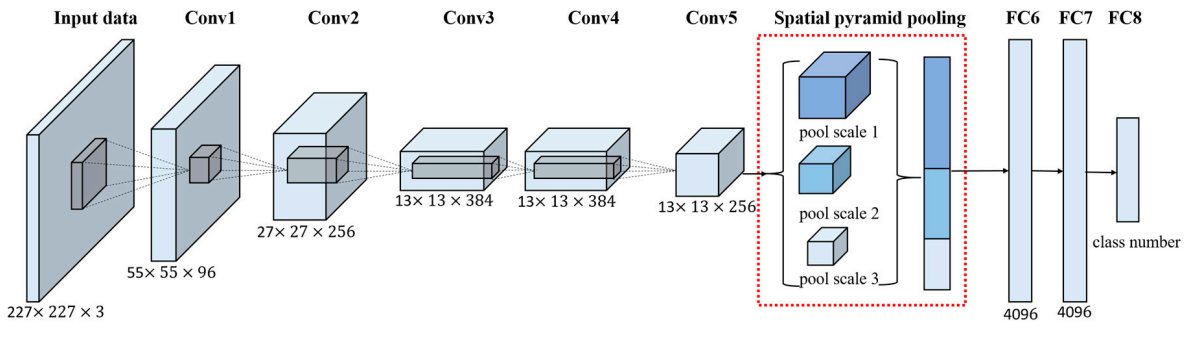
\includegraphics[height = 4.35cm, width= 12cm]{alexnet2.PNG}
\newline
From there we can use the AlexNet to have the machine actually learn to solve problems instead of just simply memorizing them. While you can ace a test just simply knowing what the answers are, it is more important for you to understand why the answers right to truly master what the test truly is. The same goes with machines, you can easily have a computer memorize by uploading data to the computer with a flash drive or download data to the computer online, but to have it learn how to download or even detect the data is a whole different process. This is where the AlexNet serves its purpose by through detecting certain parts of images can actually make the machine learn why and how a certain pattern pixels are on an image, as opposed to simply memorizing that it is there.
\newline
\newline
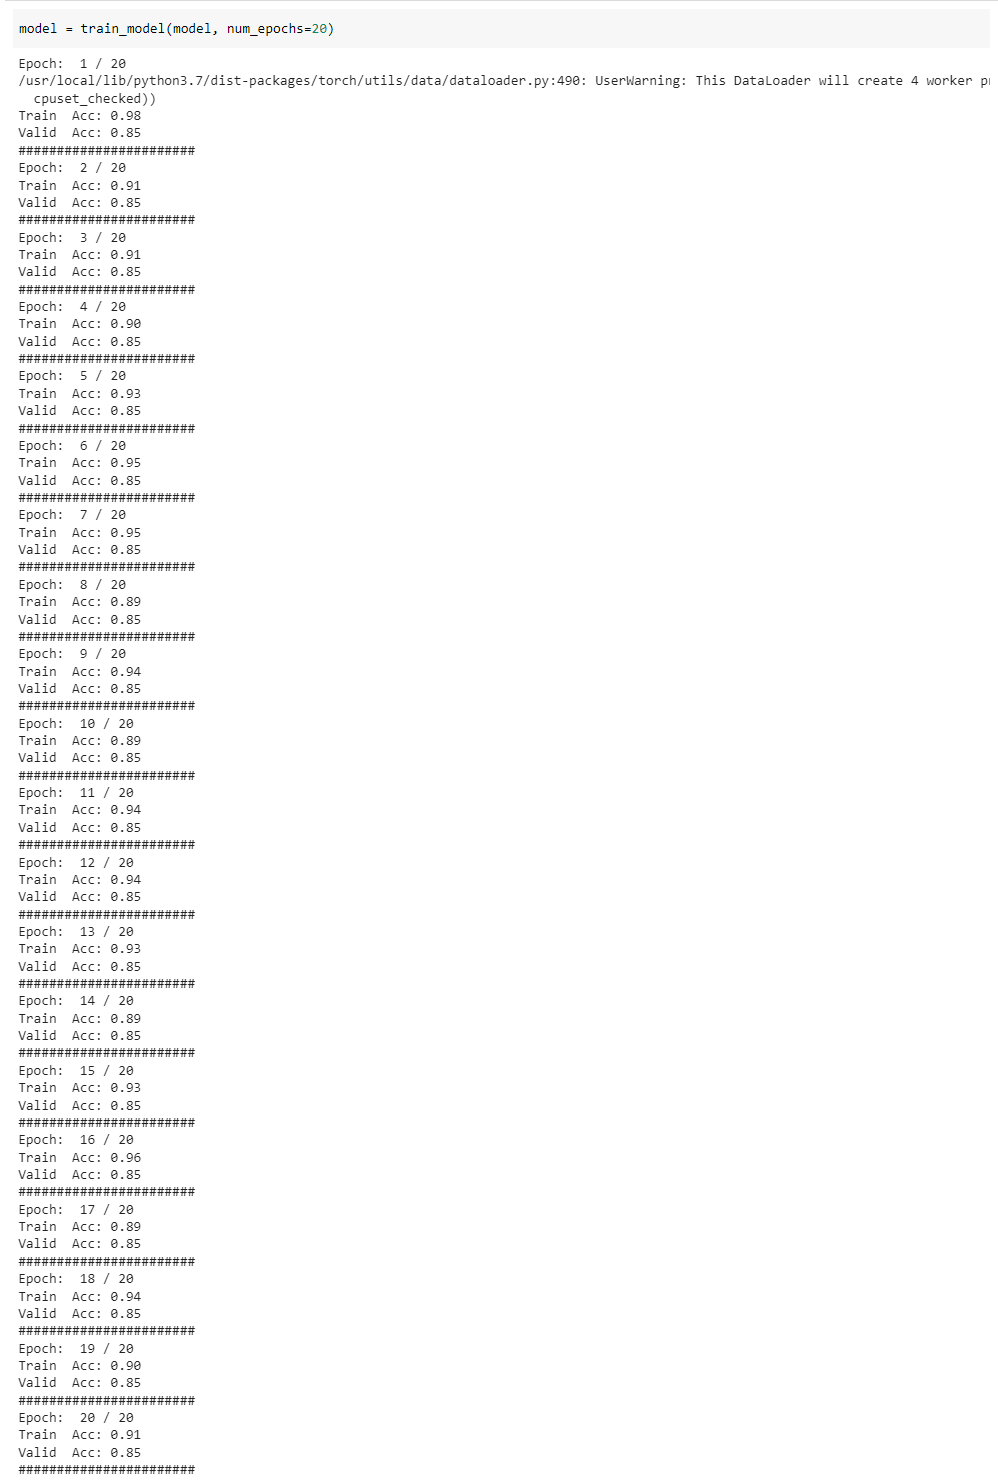
\includegraphics[height = 15cm,width=7.5cm]{training.PNG}
\newline


Because the machine or Artificial Intelligence is learning as opposed to simply memorizing why a certain pattern of pixels, which are red and green traffic lights in our case, in certain tougher situations it isn't always accurate. That is what truly makes the AlexNet a machine learning architecture as opposed to a typical machine memory which would of course be 100 percent accurate. The AlexNet also first trains the machine or AI through 80 red amd green light images named  'train' in our case, which is usually more accurate. Then the AlexNet goes through the test which is called 'valid' which tests the machine to see if it can choose the right traffic light color. Usually because of the intense training the AI is given (and the code made for the AlexNet is right), the AlexNet can easily get the images right. However since the machine is learning and not memorizing, it misses the mark of the color lights occasionally and then gets it wrong. 
\newline
\newline
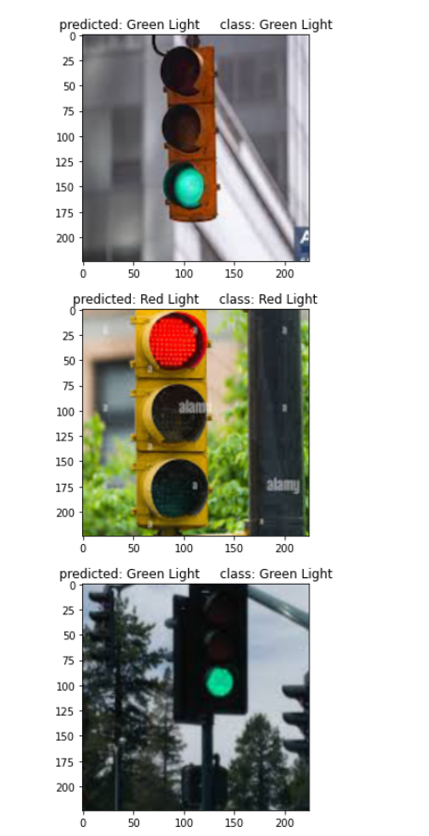
\includegraphics[height =6.25cm,width=3.5cm]{pictures result1.PNG}
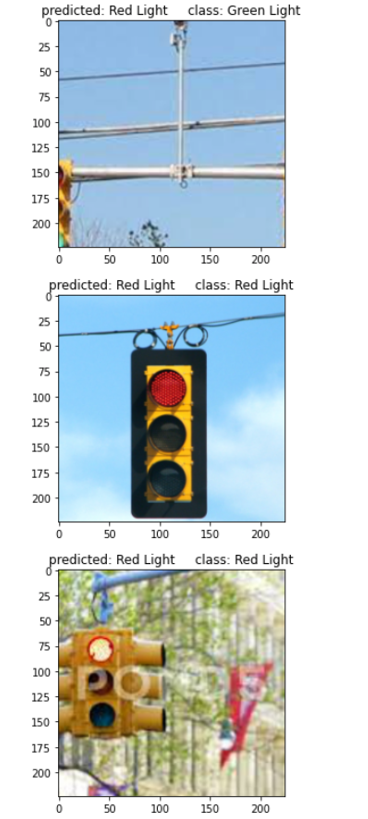
\includegraphics[height =6.25cm,width=3.5cm]{pictures result2.PNG}
\newline
\newline
The power AI through machine learning using the AlexNet Architecture, can't be underestimated as it in some ways emulates the brain of a 4 year old human being who is simply learning how to differentiate what is a green or red light on the street to know when the driver can pass the intersection or not. The same applies to self driving cars such as Teslas who have to do machine learning on a similar level, in order to determine when to move or stop based on traffic lights, car traffic and other obstacles. There are so many other things you can have the AlexNet architecture make the machine learn to differentiate with two or more images, including facial recognition, fingerprint scanners, credit card verification, and many more purposes. There are limitless possibilities to what you can do with the AlexNet Architecture for machine learning.
\chapter{References}
\label{References}
\thispagestyle{empty}

Han, Xiaobing, Yanfei Zhong, Liqin Cao, and Liangpei Zhang. 2017. "Pre-Trained AlexNet Architecture with Pyramid Pooling and Supervision for High Spatial Resolution Remote Sensing Image Scene Classification" Remote Sensing 9, no. 8: 848. https://doi.org/10.3390/rs9080848





% $$$$$$$$$$$$$$$$$  include Appendices   $$$$$$$$$$$$$$

		



\end{document}

